%========================%
%        Preamble        %
%========================%
\documentclass[12pt]{amsart}

    %========================%
%        Packages        %
%========================%

\usepackage[utf8]{inputenc}
%\usepackage{amsmath}    % Included in amsart package
%\usepackage{amsthm}     % 
\usepackage{amssymb}      % 
\usepackage{mathtools}      % Paired Limiter Macros
% \usepackage{mdframed}       % boxes for theorem
\usepackage{enumitem}     % Continuous numbering of lists
\usepackage[hidelinks]{hyperref}
\usepackage{tikz}
\usetikzlibrary{positioning}
\usepackage{blindtext}
\usepackage{graphicx}
\usepackage{float}

%========================% 
%          Title         %
%========================% 
\title{Chapters 21 and 22 Notes}
\author{Anish Sundaram}
\date{\today}

%========================% 
%        Theorems        %
%========================% 
\theoremstyle{definition}
\newtheorem{theorem}{Theorem}  % Boxed theorems
\newtheorem{definition}{Definition} % Definitions
\newtheorem{example}{Example}       %
\newtheorem{algorithm}{Algorithm}
\newtheorem*{proof*}{Proof}         % non-numbered
\newtheorem*{remark}{Remark}        %
\numberwithin{equation}{theorem}    % Local equation numbering

\setcounter{tocdepth}{3}      % Show subsubsections in contents

%========================% 
%        Macros          %
%========================% 
\DeclarePairedDelimiter\abs{\lvert}{\rvert}  % Vertical bars
\DeclarePairedDelimiter\norm{\lVert}{\rVert} % Double vertical bars
\newcommand{\drawvec}[1]{                    % matrices on one line
    \begin{bmatrix}
        #1
    \end{bmatrix}
}


% \begin{figure}[H]
%     \centering
%     \includegraphics[width=5in]{global-carbon-cycle.png}
%     \caption{The Global Carbon Cycle}
%     \label{global-carbon-cycle}
% \end{figure}

%========================% 
%         Document       %
%========================% 
\begin{document}

\maketitle

\tableofcontents

\section*{21 Electric Charge and Electric Field}
Electromagnetic interactions involve particles that have electric charge, 
an attribute that is as fundamental as mass. Just as objects with mass are 
accelerated by gravitational forces, so electrically charged objects are 
accelerated by electric forces.


\subsection*{21.1 Electric Charge}
\begin{definition}
    \textbf{Electric Charge}: 
    is the state of having more or less than a natural
    amount of electrons.\textit{Positive} if less or \textit{Negative} if more. 
    \begin{remark}
        Two positive charges or two negative charges repel each other. A 
        positive charge and a negative charge attract each other.
    \end{remark}
\end{definition}

\begin{definition}
    \textbf{Electrostatics}: 
    the interactions between electric charges that are 
    at rest (or nearly so).
\end{definition}

\subsubsection*{21.1.1 Electric Charge and the Structure of Matter}

\begin{definition}
    \textbf{Parts of Atom}: 
    Positive Protons, negative Electrons and Neutral 
    Neutrons. Protons and Neutrons are held by \textit{Strong Nuclear Force} 
    to form the Nucleus and are themselves comprised of \textit{Quarks}. 
    The majority of Atom is the \textit{Electron Cloud}
\end{definition}

\begin{definition}
    \textbf{Ionization}: 
    Normally positive charge and negative charge cancel 
    out, but through an addition or loss of an electron the atom becomes 
    ionized, becoming either a \textit{positive} or \textit{negative} ion 
\end{definition}

\begin{figure}[H]
    \centering
    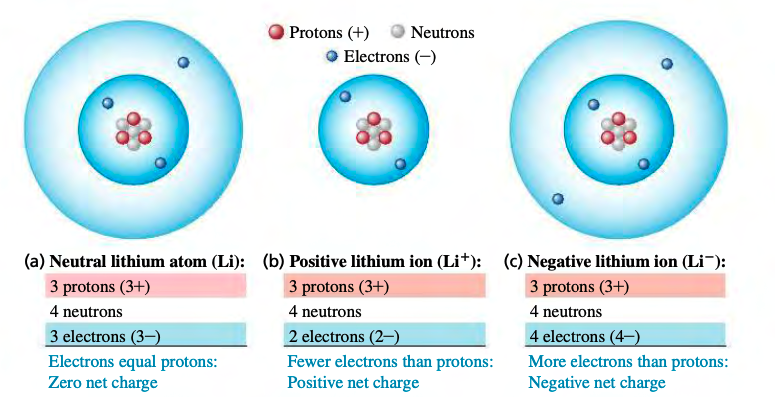
\includegraphics[width=5in]{Media/Atomic.png}
    \caption{Atomic Structure and Ionization}
    \label{Atomic Structure and Ionization}
\end{figure}

\subsubsection*{21.1.2 Electric Charge is Conserved}

\begin{theorem}
    \underline{Principle of conservation of charge}:
    The algebraic sum of all the electric charges in any closed system is 
    constant. In any charging process, charge is not created or destroyed; 
    it is merely transferred from one body to another.
\end{theorem}

\begin{theorem}
    \underline{Quantized Nature of Charge}:
    The magnitude of charge of the electron or proton is a natural unit of charge.
\end{theorem}

\subsection*{21.2 Conductors, Insulators, and Induced Charges}
\begin{definition}
    \textbf{Conductivity and Insulation}: 
    \textit{Conductors} are materials that transfer electrons well, such as 
    copper and other metals. The opposite are \textit{Insulators} which are 
    poor and transfering charge, these are often nonmetals. Some materials 
    called \textit{Semiconductors} are intermediate in their properties between
    good conductors and good insulators.
\end{definition}

\subsubsection*{21.2.1 Charging by Induction}

\begin{definition}
    \textbf{Induction}: 
    a method used to charge an object without actually touching the object to 
    any other charged object. This is done by rearranging electrons already 
    present in object
\end{definition}

\begin{definition}
    \textbf{Polarization}: 
    The slight shifting of charge within the molecules of the neutral insulator
    when placed near a charge object. This is what causes charge by Induction
\end{definition}

\begin{figure}[H]
    \centering
    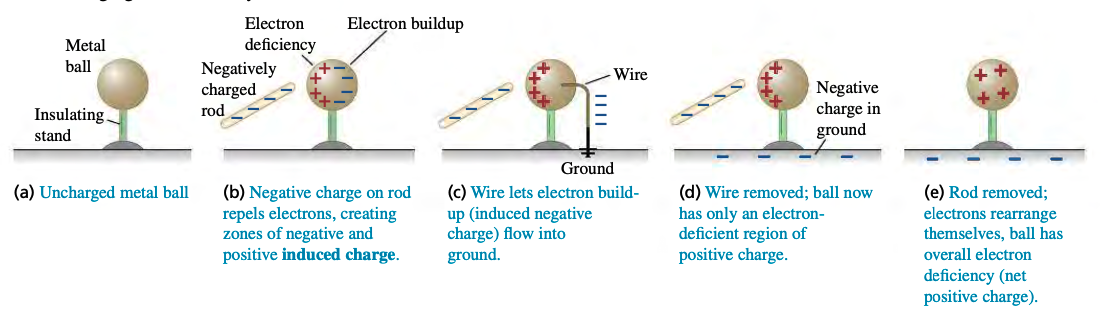
\includegraphics[width=5in]{Media/Induction.png}
    \caption{Charge by Induction}
    \label{Charge by Induction}
\end{figure}

\subsection*{21.3 Coulomb's Law}
\begin{definition}:
    \textbf{Point Charges}:
    Simple charged bodies whose mass is irrelevant.
\end{definition}

\begin{theorem}
    \underline{Coulomb's Law}: The magnitude of the electric force between two 
    point charges is directly proportional to the product of the charges and
    inversely proportional to the square of the distance between them.
    In mathematical terms shown as $$F=k\frac{|q_1*q_2|}{r^2}$$ 
    where the coulomb constant k = $8.987551787*10^9 N \cdot m/C^2$ and can 
    also be described in SI units as $\frac{1}{4\pi\epsilon_0}$.
\end{theorem}

\begin{theorem}
    \underline{Principle of Superposition of Forces}: To find sum of forces a 
    vector sum must be calculated involving the composite internal forces.
\end{theorem}

\begin{figure}[H]
    \centering
    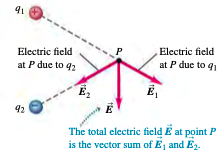
\includegraphics[width=5in]{Media/superposition.png}
    \caption{Superposition}
    \label{Superposition}
\end{figure}

\subsection*{21.4 Electric Field and Electric Forces}

\begin{definition}
    \textbf{Electric Field}:
    The intermediary through which charges interact. 
    The equation to find the strength of an electric field is $$|E| = \frac{1}{4\pi\epsilon_0}\frac{q}{r^2}$$
    where the sign relates to the direction of the field.
    \begin{remark}
        The electric force on a charged body is exerted by the electric field 
        created by other charged bodies.
    \end{remark}
\end{definition}

\subsection*{21.5 Electric-Field Calculations}

\begin{theorem}
    \underline{Principle of Superpositon of Electric Fields}:The total electric 
    field at P is the vector sum of the fields at P due to each point charge 
    in the charge distribution. 
\end{theorem}

\begin{definition}
    \textbf{Types of Charge Density}: 
    \begin{enumerate}
        \item Linear Charge Density: Charge per unit length, measured in $C/m$
        and written as $\lambda$
        \item Surface Charge Density: Charge per unit area, measured in $C/m^2$ 
        and written as $\sigma$
        \item Volume Charge Density: Charge per unit volume, measured in 
        $C/m^3$ and written as $\rho$.
    \end{enumerate}
\end{definition}

\subsection*{21.6 Electric Field Lines}
\begin{definition}
    \textbf{Electric Field Line}:
    An imaginary line demonstrating direction of 
    electric field |E| vector at point and the density of lines shows magnitude.
\end{definition}

\begin{figure}[H]
    \centering
    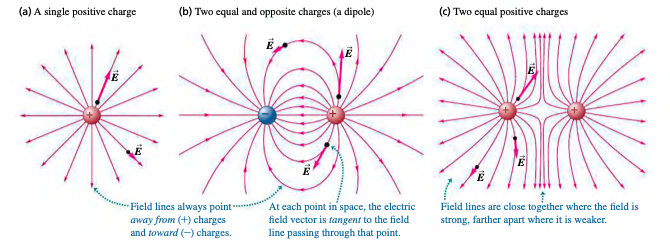
\includegraphics[width=5in]{Media/Fieldline.png}
    \caption{Field Lines}
    \label{Field Lines}
\end{figure}

\subsection*{21.7 Electric Dipoles}

\begin{definition}
    \textbf{Electric Dipole}:
    A pair of point charges with equal magnitude and 
    opposite sign (a positive charge q and a negative charge -q) separated by a
     distance d.
\end{definition}

\subsubsection*{21.7.1 Force and Torque on an Electric Dipole}

\begin{definition}
    \textbf{Electric Dipole Moment}:
    A measure of the system's overall polarity,
    can be calculated using $$p = qd$$ where q is charge and d is seperation.
    
    \begin{remark}
        Direction of p is from negative to positive
    \end{remark}
\end{definition}

\begin{definition}
    \textbf{Torque on an Electric Dipole}:
    Because the point charges may not be
    parallel, a torque exists and can be found through the equation $$\tau = pEsin\phi$$
    where p is the dipole moment and $\phi$ is the angle between the dipole moment and E
\end{definition}

\begin{definition}
    \textbf{Potetial Energy of an Electric Dipole}:
    Because there is work being
    there is a change in potential energy and we can find this through the equation
    $$U =-p\cdot E = pEcos\phi$$ 
\end{definition}

\section*{22 Gauss's Law}
 Here’s what Gauss’s law is all about. Given any general distribution of charge,
 we surround it with an imaginary surface that encloses the charge. Then we 
 look at the electric field at various points on this imaginary surface. 
 Gauss’s law is a relationship between the field at all the points on the 
 surface and the total charge enclosed within the surface.

 \begin{definition}
    \textbf{Closed Surface}:
    An essential part of making a calculation of flux,
    The shape must entirely enclose a volume to calculate Gauss's Law.
\end{definition}


 \subsection*{22.1 Charge and Electric Flux}

\begin{definition}
    \textbf{Electric Flux}: 
    the rate of flow of the electric field through 
    a given area. Electric flux is proportional to the number of 
    electric field lines going through a virtual surface. Independent of size.

    \begin{remark}
        Positive charge inside the box goes with an outward electric flux 
        through the box’s surface, and negative charge inside goes with an 
        inward electric flux. If there is no charge, neto zero charge, or the 
        same flux in and out there is no electrix flux. 
    \end{remark}
\end{definition}

\subsection*{22.2 Calculating Electric Flux}

\begin{definition}
    \textbf{Flux of Uniform Electric Field}:
    Flux exists as the overlap of the
    electric field and the surface. Mathematically it is expressed as 
    $$\Phi_E = EAcos\phi$$ where $\phi$ is the vertical angle normal to the surfaces.
\end{definition}

\begin{figure}[H]
    \centering
    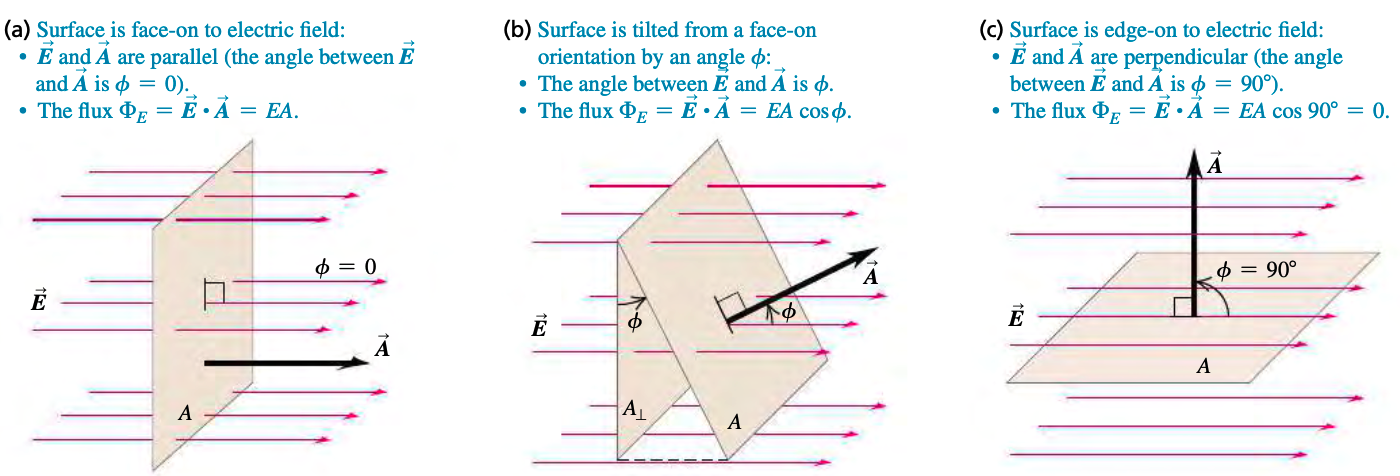
\includegraphics[width=5in]{Media/Uniformflux.png}
    \caption{Uniform Flux}
    \label{Uniform Flux}
\end{figure}

\begin{definition}
    \textbf{Flux of Nonuniform Electric Field}:'
    To find the flux of a varying electric field or on a curved survace we must
    find the surface integral by finding an infintesimal dA.For this case the 
    equation morphs to $$\Phi_E = \int EAcos\phi dA = \int E \cdot dA$$ where 
    $\phi$ is again the vertical angle normal to surface and A is surface area.
\end{definition}

\subsection*{22.3 Gauss's Law}

\begin{theorem}
    \underline{Gauss's Law}:
    An alternative to Coulomb's Law, Gauss's law states the total electric flux
    through a closed surface is proportional to total net electric charge. The
    complete relation can be read as 
    $$\Phi_E = \int EA cos\phi = \frac{1}{4\pi \epsilon_0} \frac{q}{R^2}(4\pi R^2) = \frac{q}{\epsilon_0}$$
    for a sphere, noting that flux is independent of Radius, only charge $q$


    \begin{remark}
        General Form of Gauss's Law can be expressed as The total electric 
        flux through a closed surface is equal to the total (net) electric 
        charge inside the surface, divided by $\epsilon_0$, or in equation form 
        $$\Phi_E = \frac{Q_encl}{\epsilon_0}$$
    \end{remark}
\end{theorem}


\pagebreak

\section*{Important Equations}


\textbf{Electric Fields and Charge Density}

\textbf{Gauss's Law and Flux}

\end{document}